\documentclass[a4paper,12pt]{article}
% Use the options 'crop' to show crop marks, and
% 'doublespaced' for double line spacing.
% e.g. \documentclass[crop,doublespaced]{cupjournal}


%calling packages
\usepackage[english]{babel}
\usepackage[utf8]{inputenc}
\usepackage{amsmath}
\usepackage{graphicx}
\usepackage[left=1in,right=1in,top=1in,bottom=1in]{geometry}
\usepackage{setspace}
\usepackage[round,sort]{natbib}
\usepackage{epstopdf}
\usepackage{soul}
\usepackage{lmodern}
\usepackage{caption}
\usepackage{hyperref}
\usepackage{subcaption}
\usepackage{rotating}

\usepackage{etoc}


\usepackage{xr}
\externaldocument{"appendix"}


\usepackage{longtable}
\usepackage{amssymb}
\usepackage{fancyhdr}
\usepackage{array}
\usepackage{pdfpages}
\usepackage{lscape} % for landscape formatting of pages
\newcolumntype{P}[1]{>{\centering\arraybackslash}p{#1}}
%fonts
\usepackage{times}
%\setcounter{secnumdepth}{0}
%chanfing font of table headers
\captionsetup[figure]{labelfont=bf}
\captionsetup[table]{labelfont=bf}

%path to where figures are located
\graphicspath{ {images/} }

%for notes in table captions 
\newcommand\fnote[1]{\captionsetup{font=small}\caption*{#1}}

%changing header
\pagestyle{fancy}
\fancyhf{}
\rhead{\thepage}
\renewcommand{\headrulewidth}{0pt}
\renewcommand{\footrulewidth}{0pt}
%set spacing

\renewcommand{\sfdefault}{phv}

\doublespacing
\usepackage{titlesec}

\titleformat*{\section}{\Large\sffamily}
\titleformat*{\subsection}{\large\sffamily}
\titlespacing*\section{0pt}{24pt plus 4pt minus 2pt}{4pt plus 2pt minus 2pt}
\titlespacing*\subsection{0pt}{20pt plus 4pt minus 2pt}{4pt plus 2pt minus 2pt}


%changing title settings
\makeatletter
\renewcommand{\maketitle}{
	\begin{flushleft}
		
		\onehalfspacing
		
		\@title
		
		\lineskip .5em
		\normalfont{\normalsize{\@author}}
\end{flushleft}}
\makeatother


\newcommand{\beginsupplement}{%
	\setcounter{table}{0}
	\renewcommand{\thetable}{S.\arabic{table}}%
	\setcounter{figure}{0}
	\renewcommand{\thefigure}{S.\arabic{figure}}%
}


%title
\title{\bigskip \bigskip \sffamily \LARGE{Can Citizens Set City Policy?} \\ \Large{ Evidence From A Decentralized Welfare State}}

%author
\author{\bigskip Benjamin Carl Egerod\thanks{Graduate Student, Department of Political Science, University of Copenhagen, e-mail: \texttt{benjamin.carl.egerod@ifs.ku.dk}.} \qquad Martin Vinæs Larsen\thanks{Assistant Professor, Department of Political Science, Aarhus University, e-mail: \texttt{mvl@ps.au.dk}.}} 



\begin{document}

	
\begin{footnotesize} \noindent \today. \end{footnotesize} %date

\vspace{0.7in}

\maketitle

\bigskip

\begin{quotation} %abstract
	
	\small \noindent \emph{Abstract:} Municipal governments supposedly empower citizens, giving them the ability to shape the political organization of their local community. In spite of this, we know little about whether municipal governments are in fact responsive to the policy views of municipal electorates. In this study, we look at whether the policy implemented by local politicians actually respond to changes in the public mood. To do this, we compile a unique and comprehensive dataset of local fiscal policy, which we use to construct municipal-level estimates of fiscal policy conservatism. This detailed policy data is then linked to an indicator of local ideological sentiment. We find strong evidence for dynamic responsiveness: when preferences in a municipality changes, public policy responds.
\end{quotation}




\thispagestyle{empty} %removing page number from page one


\clearpage

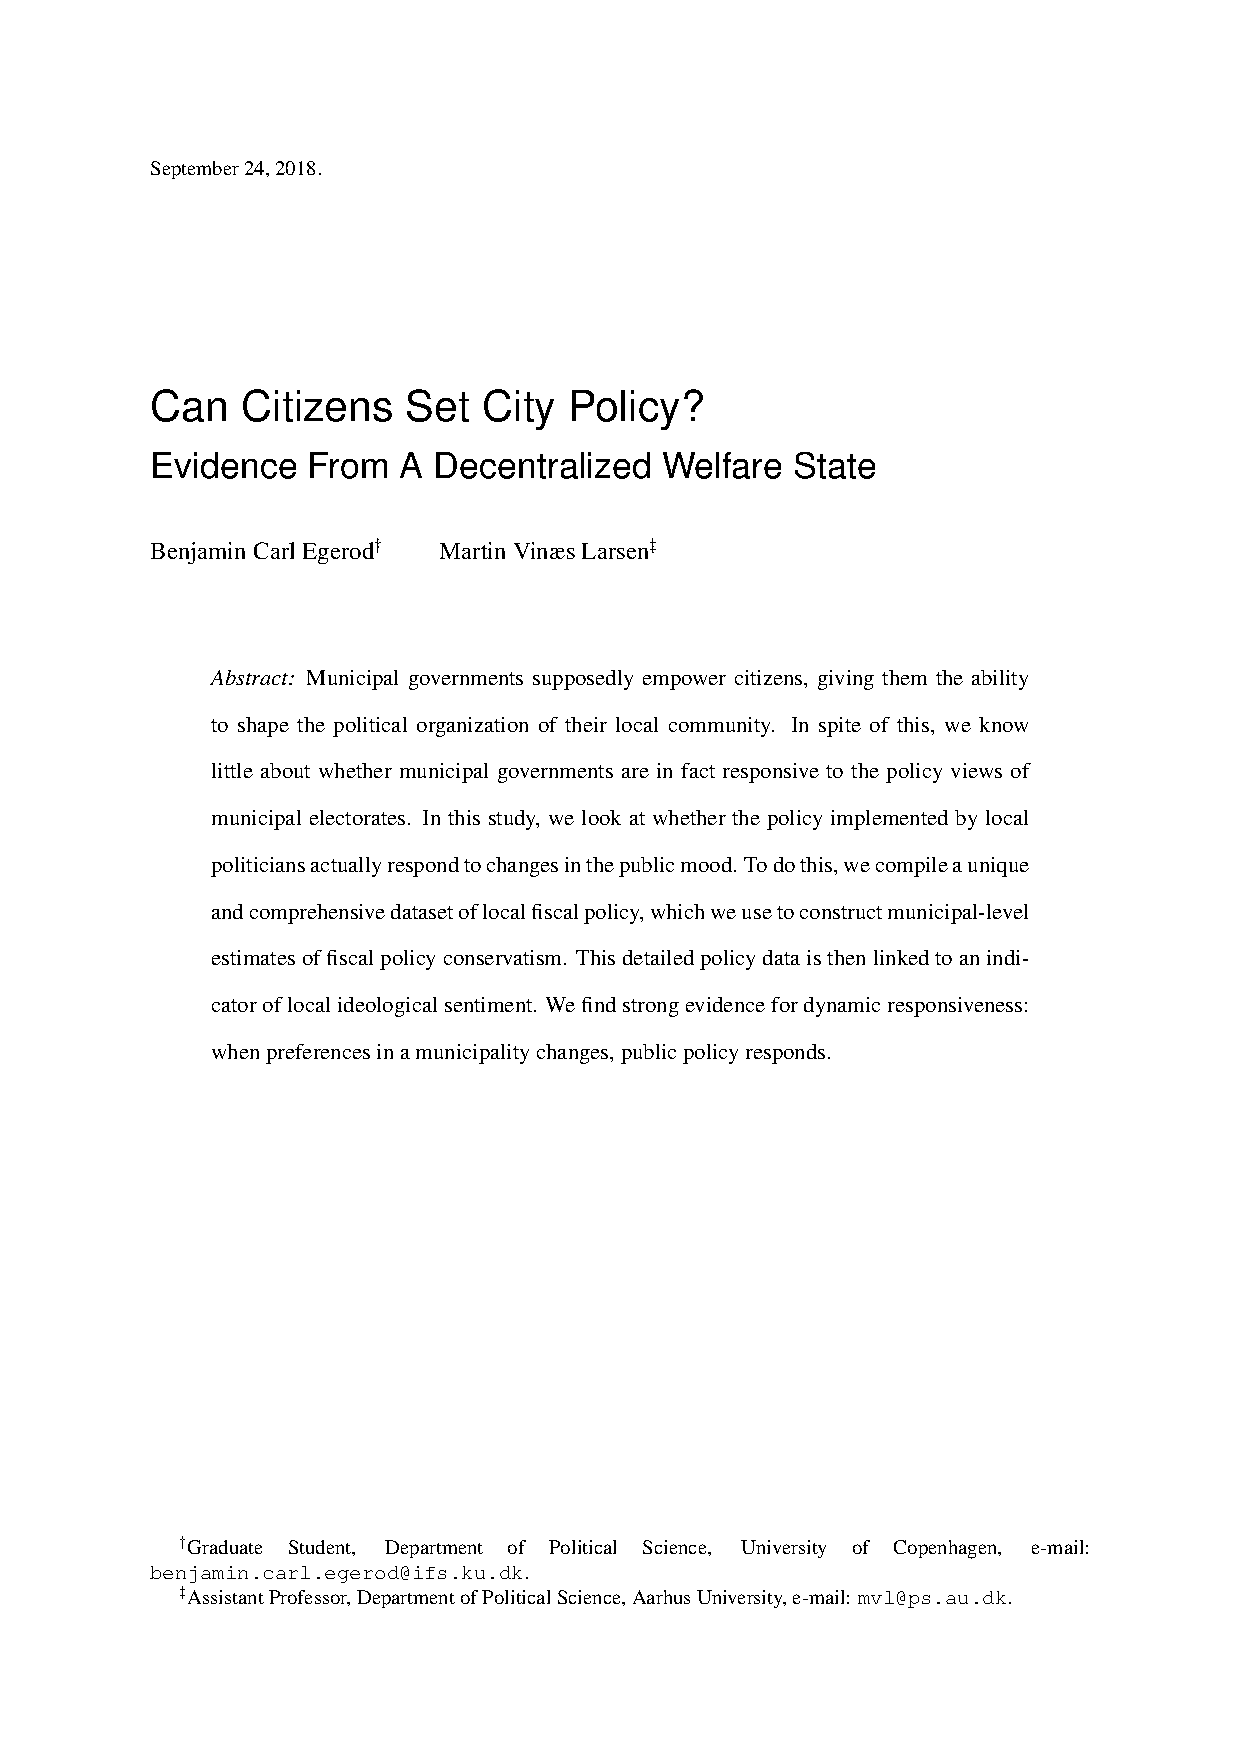
\includepdf[pages=-]{citypolicy_vol2}

\clearpage
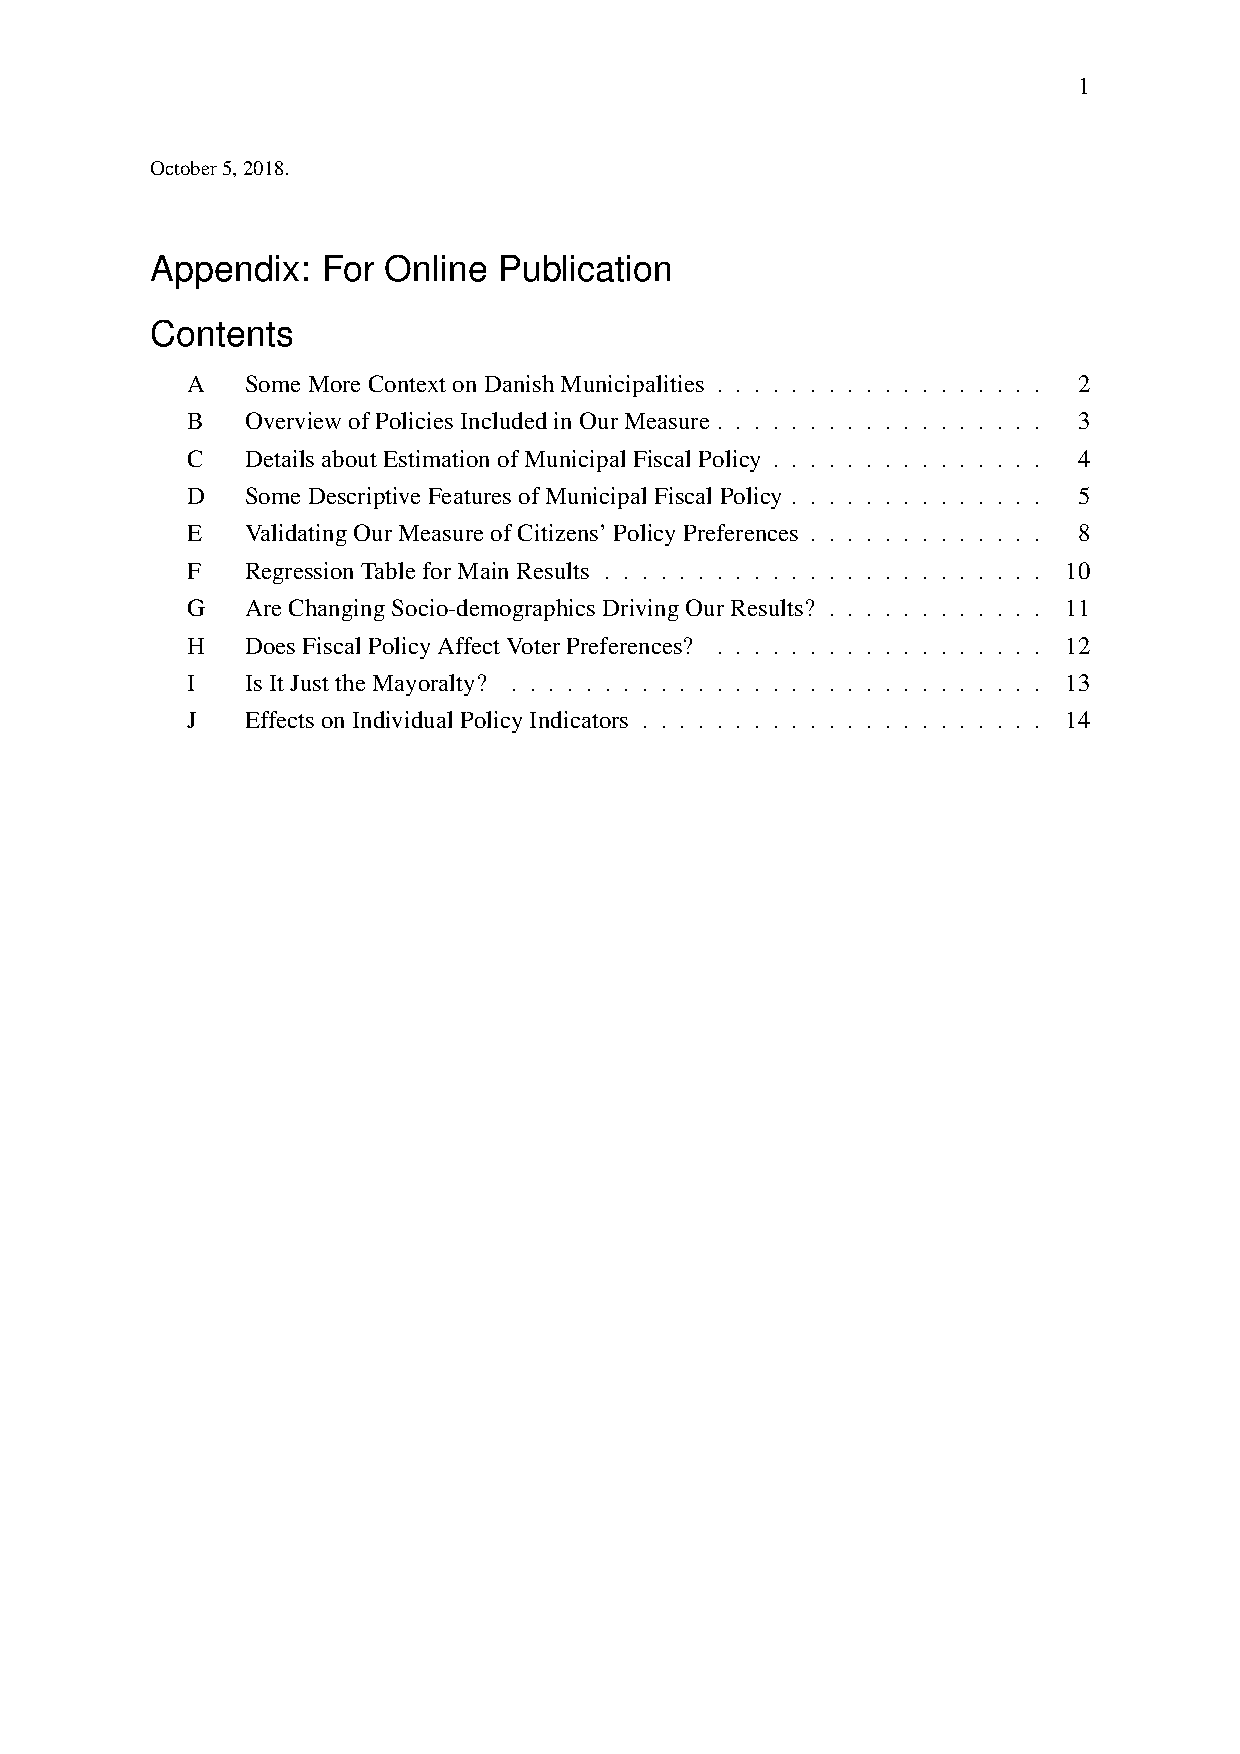
\includepdf[pages=-]{appendix}


\end{document}

